\section{INTRODUCTION}
The last decade has seen a massive explosion of on-line data in all forms be it news articles, blogs or social media like Twitter, Facebook and MySpace.
Twitter is a novel micro-blogging service and was launched in 2006.
Twitter users post messages called tweets on a public message board  and these tweets are limited to 140 characters.
Originally the tweets were meant to be personal status updates but over the years these tweets have evolved into much more.
Now apart from simple status updates, tweets can be URLs websites or even directed messages to particular individuals.
Due to the short nature of the messages users often combine multiple words into \emph{hashtags} to convey their views.
Therefore, these hashtags become the most important part of a tweet as the entire essence of the tweet is captured in single hashtag.. 
These hashtags evolve over time and gain more traction as users adopt the popular ones.
This makes the language used in Twitter very different from other textual web content like blogs and articles.
\newline
Today twitter has grown so big\footnote{As of May 7,2013 twitter has 555 million active registered users with 135000 new users signing up everyday and approximately 1 billion tweets created every 5 days}
that it has come to be looked at as a treasure trove of mine-able data.
With official APIs that are open to public, the easy access to large volumes of data has piqued the interest of scientists in the data mining community.
Researchers have studied various real world phenomenon like book sales, box office earnings and even stock prices and have not only shown that they have  strongs correlations to the chatter on Twitter ~\cite{gruhl2005predictive,asur2010predicting,bollen2011twitter}
but were also able to make forecasts about future trends too.
\paragraph{}
However, the more curious research is whether the on-line chatter be used to model the social, economic and political landscape of a country.
Political leaders have started using Twitter as a channel to mobilize supporters for their ideologies.
For the 2008 US presidential election Barack Obama used social media and specifically Twitter extensively in his campaign. 
His victory established Twitter as a channel to garner support for a particular idealogy be it political or otherwise.
Bollen et al. ~\cite{bollen2011modeling} used a version of the well-established psychometric instrument- Profile of Mood States(POMS) to model the mood of twitter traffic and correlate it to a number of social and economic events that occurred during the same time period. 
The results from this research instigated more researchers to study and quantify the political sentiment through social media and if possible even forecast election results.
However, there is a constant debate among political scientists on whether Twitter can be used as a surrogate for political opinion of the masses.
Some believe twitter indeed is an indicator of political opinions, while others question the validity of such results.. 
In this work we aim to answer these questions by trying to improve the performance of election prediction algorithms that use Twitter.
The following section reviews the current state of the art approaches to election prediction. 

\section{RELATED WORK}
We divide the literature review into four parts.
First we look at a selection of volume based approaches to predict elections i.e., models that predict election results by merely counting the number of times a particular candidate is mentioned in Twitter.
Then we review more sophisticated approaches that model the demographics of an election to make more informed predictions.
In the third section, we shall summarize a quite prevalent pessimistic view on such methodologies' capability to predict elections.
Lastly we review Probabilistic Soft Logic, a framework we use to build a vocabulary dynamically.
\subsection{Volume based approaches}
In one of the most cited papers in this space, ~\cite{tumasjan2010predicting} the authors claim that 
\emph{ "The mere number of tweets reflect voter preferences and comes close to  traditional polls.."}
while predicting  the 2010 German federal election. % by counting candidate mentions on twitter.
They go on to strongly conclude that Twitter can indeed be a valid indicator of political opinion.
This was followed by ~\cite{o2010tweets,saez2011total,bermingham2011using,demartini2011analyzing} all of which use volume based approaches combined with sentiment analysis.
Both ~\cite{o2010tweets,bermingham2011using} fit a regression model to opinion polls with volume of mentions and sentiment as independent variables and the opinion polls as the dependant variable. 
They conclude that sentiment is a weak predictor compared to share of volume.
\newline In general the methodologies described in these publications count the occurrence of certain hand filtered keywords in the "Twittersphere" and classify such tweets as positive or negative using a classifier trained on human annotated lexicons.
Some advanced sentiment classifiers also provide the likelihood that given sample of text belongs to an empirically defined psychological and structural categories like anxiety, anger, sadness etc.

\subsection{Profile Modelling}
More sophisticated approaches are adapted in ~\cite{livne2011party,conover2011predicting,diaz2012taking}. 
The authors either model the candidates or the voters in the elections rather than compute the aggregated sentiment of the mass.  
In~\cite{conover2011predicting} the authors build a Support Vector Machine classifier trained on manually labelled tweets and classify users into 'left' and 'right' aligned.
Through latent semantic analysis they claim to have identified the hidden structure in the data that is strongly associated with the users' political affiliations.
%Using this information and how political information diffuses in a network, they show  an accuracy of 95\%  in predicting the political alignment of twitter users.
Livne et al. in ~\cite{livne2011party} analyse the Twitter profiles of candidates who contesting in the 2010 mid-term elections in the U.S. 
They identify topics specific to groups of candidates, split according to their known political orientations and use the features obtained as inputs to a regression model to predict the elections. 
In a similar technique Diaz-Aviles in ~\cite{diaz2012taking} model the candidates by building a emotional vector for each candidate by using the mentions of that candidate and sentiments associated with each mention learnt using the NRC EmotionLexicon(EmoLex). 
They use these profiles to predict the rise and fall of a candidate's popularity. 

In another research, Mustafaraj et al. ~\cite{mustafaraj2011vocal} model the distribution of political content among Twitter users. 
They divide the users into two groups the "vocal minority" and the "silent majority". 
They observe that these two groups engage in different ways in social media.
The vocal minority aim to broaden the impact of tweets by re-tweeting and linking to other web-content whereas the silent majority who tweet significantly lesser are more inclined to share their personal view points.
Though they do not make any predictions about elections, they make very valid observations such as 
\emph{"Because of this differences between content generated by different groups , one should be aware of aggregating data and building models upon them, without verifying the underlying model that has generated the data."}.

\subsection{Flaws in current state of the art}
Of late there has been a lot of studies showing how such models that predict elections using social media feeds are flawed ~\cite{metaxas2011not,gayo2012wanted,gayo2011don,gayo2011limits}.
These publications not only list the obvious issues in using Twitter to predict elections but also detail recommendations on how to make such methodologies better.
Daniel Gayo-Avello surveys almost all the state of the art approaches in predicting elections in his paper ~\cite{gayo2012wanted} most of which is detailed above.
According to him post-hoc analysis of elections in retrospect must not count as valid predictions and also states that researchers do not report negative results leading to what is called the \emph{file drawer} effect. 
His major points of argument against such models are:
\begin{itemize}
\item
The models are tailor made to fit a particular election and that they need to be generic enough to reproduce similar results when run on other elections.
In particular Metaxas et al in ~\cite{metaxas2011not} state that any method claiming predictive power on the basis of Twitter data should be a clearly defined algorithm and should be "explainable" i.e., black box approaches should be avoided.
\item
There is no predefined notion of "vote" that has been used to predict the elections.
Most of the models aim to predict elections merely by counting the tweets related to a candidate.
\item
Biases in Twitter are ignored. Twitter is not a representative sample of the electorate demographic as not every age gender or social group is represented.
He also notes that since people tweet on a voluntary basis the data produced is only by those who are politically active. 
Another point of contention is the credibility of tweets i.e., whether the tweets are rumours, campaign propaganda or contain misleading information just to maliciously attack candidate's on-line popularity.
\item
Since in 2008 and 2010 , 91.6\% and 84\% of elections were won by the the incumbent candidate respectively, Gayo-Avello argues that incumbency should be the baseline rather than just chance.
He also notes that most of the methodologies are only slightly better than chance.
\item
Lastly he states even though sentiment classifiers are highly researched space in Natrual Language Processing, the accuracy of such methods are only slightly better than random classifiers. 
Further, these classifiers do not detech humour and sarcasm which in his opinion plays a major role in political discussions.
%\item
%Lastly in ~\cite{gayo2011don} Gayo-Avello akin to ~\cite{mustafaraj2011vocal} states that abstaining from tweeting about politics can play even more important role than the ones mentioning the candidates and hence researches should also model this lack of chatter about a particular candidate or political party.
\end{itemize}

\subsection{Probabilistic Soft Logic}
Probabilistic Soft Logic ~\cite{kimmig2012short} is a framework for collective probabilistic reasoning on relational domains.
PSL models have been developed in various domains, including collective classification ~\cite{broecheler2010computing}, ontology alignment ~\cite{brocheler2012probabilistic}, personalized medicine ~\cite{bach2010decision}, opinion diffusion ~\cite{bach2012scaling} , trust in social networks ~\cite{huang2012probabilistic}, and graph summarization ~\cite{memory2012graph}.
PSL represents the domain of interest as logical atoms.
It uses first order logic rules to capture the dependency structure of the domain, based on which it builds a joint probabilistic model over all atoms.
Instead of hard truth values of $0$ (false) and $1$ (true), PSL uses soft truth values relaxing the truth vlaues to the interval $[0,1]$.
The logical connectives are adapted accordingly.
This makes it easy to incorporate similarity or distance functions.
\newline
User defined \emph{predicates} are used to encode the relationships and attributes and \emph{rules} capture the  dependencies and constraints.
Each rule's antecedant is a conjunction of atoms and its consequent is a disjunction. 
The rules can also labled with non negative weights which are used during the inference process. 
The set of predicates and weighted rules thus make up a PSL program where known truth values of ground atoms derived from observed data and unknown truth values for the remaining atoms are learnt using the PSL inference.
\newline
Given a set of atoms 
$\ell = \{\ell_1,\ldots,\ell_n\}$,
an interpretation defined as 
$I : \ell \rightarrow [0,1]^n$
is a mapping from atoms to soft truth values.
PSL defines a probability distribution over all such interpretaions such that those that satisfy more ground rules are more probable.
\emph{Lukasiewicz t-norm} and its corresponding co-norm are used for defining relaxations of the logical AND and OR respectively to determine the degree to which a ground rule is satisfied.
Given an interpretation $\mathit{I}$, PSL defines the formulas for the relaxation of the logical conjunction ($\wedge$), disjunction ($\vee$), and negation ($\neg$) as follows:

\begin{align*}
\ell_1 \softand \ell_2 &= \max\{0, I(\ell_1) + I(\ell_2) - 1\},\\
\ell_1 \softor \ell_2 &= \min\{I(\ell_1) + I(\ell_2), 1\},\\
\softneg l_1 &= 1 - I(\ell_1),
\end{align*}  

The interpretation $\mathit{I}$ determines whether the rules is satisfied, if not, the \emph{distance to satisfaction}.
A rule $\mathit{r} \equiv \mathit{r_{body}} \rightarrow \mathit{r_{head}} $  is satisfied if and only if the truth value of head is atleast that of the body. The rule's distance to satisfaction measures the degree to which this condition is violated.
 \newline
\begin{center} 
 $\mathit{d_r}(\mathit{I}) =$ max\{0,$\mathit{I(r_{body}} - \mathit{I(r_{head}}$\}
 \end{center}

PSL then induces a probability distribution over possible interpretations $\mathit{I}$ over the given set of ground atoms $\mathit{l} $ in the domain. 
If $\mathit{R}$ is the set of all ground rules that are instances of a rule from the system and uses only the atoms in  $\mathit{I}$ then,
the probability density function $\mathit{f}$ over $\mathit{I}$ is defined as
\begin{equation}
\label{eq:contimn1}
    f (I) = \frac{1}{Z} \text{exp}[-\sum_{r\in R} \lambda_r (d_r(I))^p]
\end{equation}
\begin{equation}
\label{eq:contimn2}
	Z = \int_{I} \text{exp} [ -\sum_{r\in R} \lambda_r (d_r(I))^p ]
\end{equation}
where~$\lambda_r$ is the weight of the rule~$r$, $Z$ is the continuous version of the normalization constant used in discrete Markov random fields, and ~$p \in \{1, 2\}$ provides a choice between two different loss functions, linear and quadratic.
The values of the atoms can be further restricted by providing linear equality and inequality constraints allowing one to encode functional constraints from the domain. 
PSL provides for two kinds of inferences (a)most probable explanation and (b)calculation of the marginal distributions. 
In the MPE inference given a partial interpretation with grounded atoms based on observed evidence, the PSL program infers the truth values for the unobserved atoms satisfying the most likely interpretation. 
In the second setting, given ground truth data for all atoms we can learn the weights for the rules in our PSL program.
\section{Motivation}
The one thing that the previously described prediction methodologies have in common is the process of filtering to obtain tweets pertaining to the particular election.
Usually this is done by a process of querying the Twitter API for a bunch of keywords such as the candidate name and political party names.
Given that the language used in twitter is completely different from the language in newspapers and magazines, this process gives a very low recall.
For example, for the 2012 presidential elections in Venezuela users preferred  the hashtags \emph{\#elmundocochavez} and \emph{\#hayuncamino} to show their support for Hugo Chavez and Henrique Capriles respectively.
Such hashtags are not known a priori and gain more traction and adaptation closer to the election.
Querying just for "chavez" or "capriles" would result in missing out on a huge chunk of tweets that are indicative of a user's political preference.
Thus it becomes vital that any methodology that predicts elections accounts for such memes that become popular during the time period leading up to the election.
% word cloud figure
\begin{figure*}[ht]
	\centering
	%\captionsetup{font=scriptsize}
	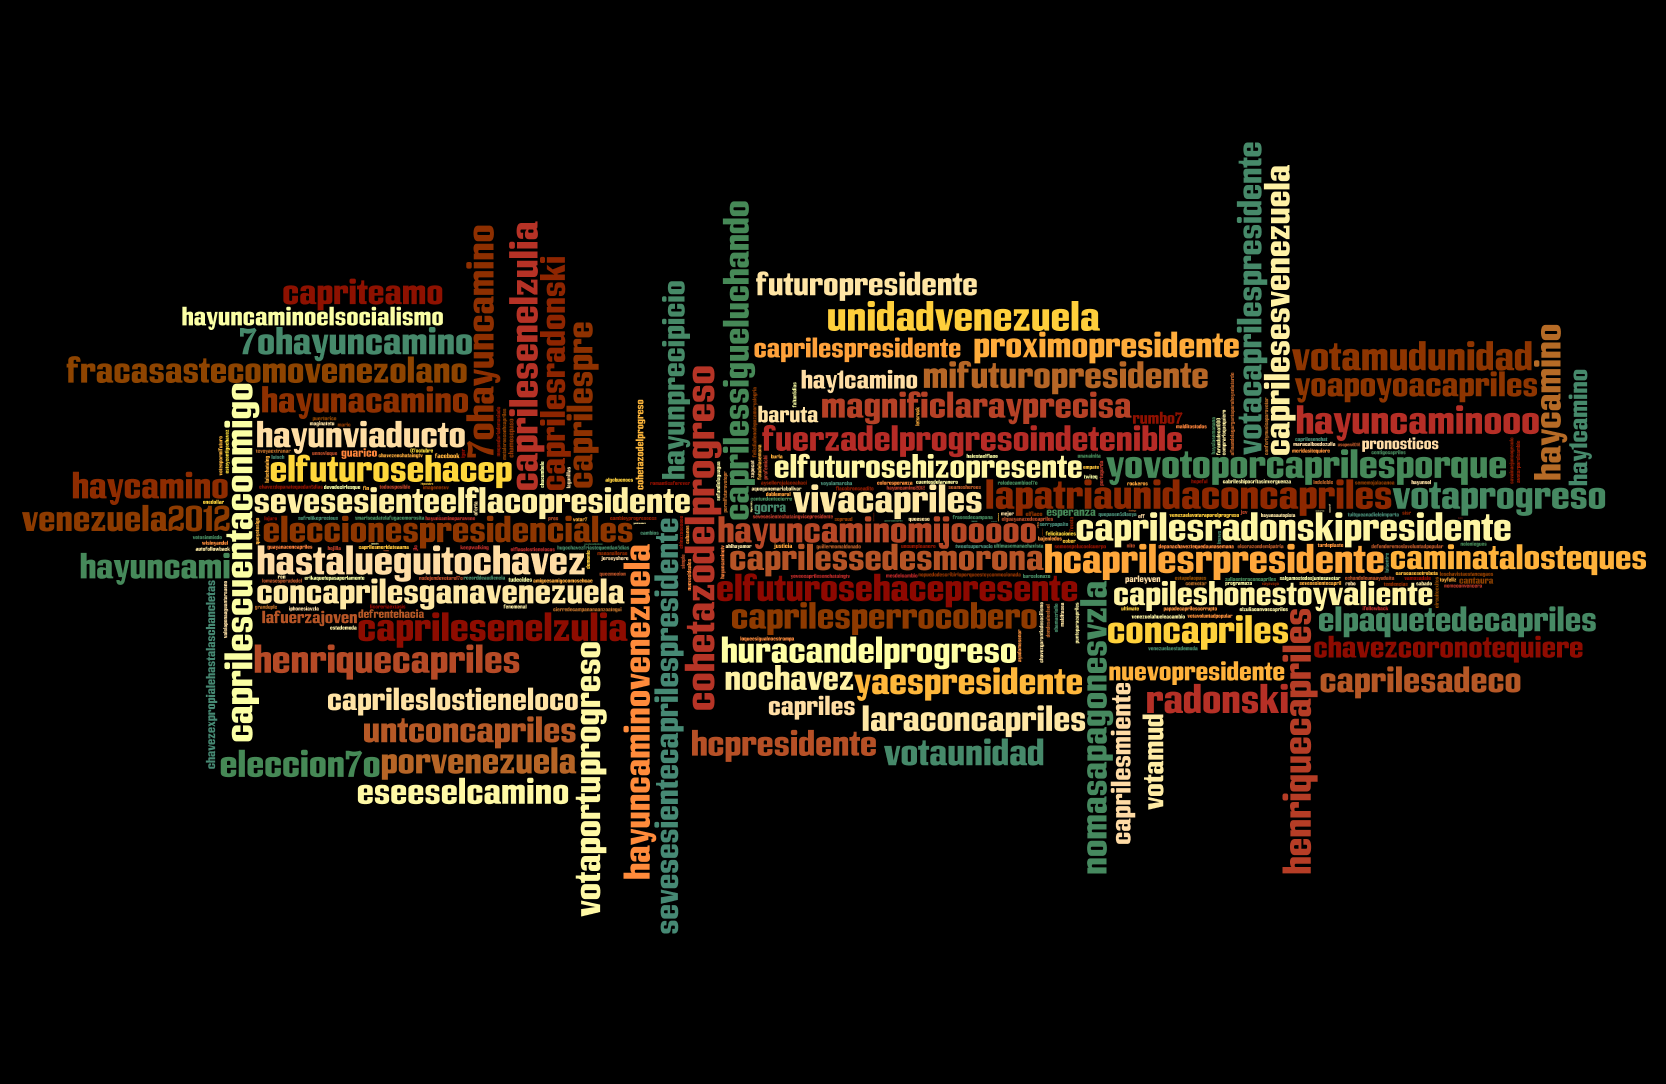
\includegraphics[width=1.0\textwidth]{support_files/caprilesWordCloud.png}
	\vspace{-1em}
	\caption{Word cloud for Henrique Capriles}
	\label{fig:caprilesWordCloud}
	\vspace{-1em}
\end{figure*}

%\newline
In this work we address this issue by building on our earlier work ~\cite{huang2012social}.
Specifically we make the following contributions:
\begin{itemize}
\item
Design and implement a new dynamic query expansion algorithm using Probabilistic Soft Logic to obtain a exhaustive vocabulary.
\item
Show how the vocabulary obtained from the Dynamic Query Expansion exercise improves the recall and accuracy of the prediction algorithms.
\end{itemize}